\section{Solutions for``Complex Numbers''}
\noindent\textbf{\textit{ (Chapter \ref{complex})}}\bigskip

%%section 2.1
\noindent\textbf{Exercise \ref{exercise:complex:root1}:}

\noindent\textbf{Exercise \ref{exercise:complex:root2}:} %kw added
%Try to use the method of Proposition~\ref{proposition:complex:no_sqrt} to prove that -4 has no real cube root. At what step does the method fail?
\begin{align*}
x^{3} &= -4		&\text{(Supposition)}\\
x &\geq 0		&\text{(Case 1,} x \geq 0)\\
x^{3} &= x \cdot x \cdot x 		&\text{(multiplication of real numbers)}\\
x^{3} &\geq 0		&\text{(multi. of pos. numbers \& multi. of 0)}\\
-4 &\geq 0		&\text{(contradictory statement)}\\
x &< 0		&\text{(Case 2,} x < 0)\\
x^{3} &< 0		&\text{(multi. of neg. numbers)}\\
-4 &< 0		&\text{(correct statement)}\\
\end{align*}
Since $-4 < 0, -4$ does have real cube roots. $-4 < 0$ is where the method fails, since it is true rather than false.\\

\noindent\textbf{Exercise \ref{exercise:complex:graph}:}

\noindent\textbf{Exercise \ref{exercise:complex:more}:}

\noindent\textbf{Exercise \ref{exercise:complex:1}:}

\noindent\textbf{Exercise \ref{exercise:complex:m2even}:}

\noindent\textbf{Exercise \ref{exercise:complex:6}:}

\noindent\textbf{Exercise \ref{exercise:complex:2}:} %KW added
%Use substitution to prove the following statement:  if $3 | n$ and $4 | m$, then $12 | mn$ (the notation ``$3 | n$'' means that 3 divides $n$). 
%\hyperref[sec:complex:hints]{(*Hint*)}
\begin{align*}
\text{If}\  3|n \text{\ and}\  4|m\text{, then}\ &		&\text{(Premise)}\\
12|mn&		\\
3|n, 4|m&		&\text{(Given)}\\
\text{Since}\ 3 \text{\ divides} \ n, n = 3j\ \text{where}\ j \in {\mathbb{Z}}\\
n = 3j&		&\text{(Def. of divisibility)}\\
\text{Since}\ 4 \text{\ divides} \ m, m = 4k\ \text{where}\ k \in {\mathbb{Z}}\\
m = 4k&	&\text{(Def. of divisibility)}\\
mn = (4k)(3j)&	&\text{(Substitution)}\\
mn = 4 \cdot 3 \cdot k \cdot k&	&\text{(multiplicative commutative law)}\\
mn = (4 \cdot 3)(k \cdot j)&	&\text{(multiplicative associative law)}\\
mn = 12kj&	&\text{(multiplication of integers)}\\
mn = 12jk&	&\text{(multiplicative commutative law)}\\
mn = 12l&	&\text{(Product of 2 integers is an integer.}\ l = jk)
\end{align*}
Since $12$ and $l$ are integers, the product is an integer as well. $12$ divides $mn$; hence, $mn = 12l$ can be written as $12|mn$ by definition.\\
$\therefore 12|mn$\\

\noindent\textbf{Exercise \ref{exercise:complex:3}:}

\noindent\textbf{Exercise \ref{exercise:complex:4}:}

\noindent\textbf{Exercise \ref{exercise:complex:5}:}

\noindent\textbf{Exercise \ref{exercise:complex:6a}:}

\noindent\textbf{Exercise \ref{exercise:complex:6aa}:}

\noindent\textbf{Exercise \ref{exercise:complex:root3}:}

\noindent\textbf{Exercise \ref{exercise:complex:7}:}

%%section 2.2
\noindent\textbf{Exercise \ref{exercise:complex:complex_associative}:}
%\\Prove that addition on complex numbers is associative.
\begin{align*}
& [(a + bi) + (c + di)] + (e + fi) &\\
&=[(a + c) + (b + d)i] + (e + fi) &\text{(complex addition)}\\
&= (a + c + e) + (b + d + f)i &\text{(complex addition)}
\end{align*}
On the other hand,
\begin{align*}
&(a + bi) + [(c + di) + (e + fi)]&\\
 &= (a + bi) + [(c + e) + (d + f)i] &\text{(complex addition)}\\
&= (a + c + e) + (b + d + f)i &\text{(complex addition)}
\end{align*}
By substitution, we get the associative property:
\[[(a + bi) + (c + di)] + (e + fi) = (a + bi) + [(c + di) + (e + fi)] \] \\

\noindent\textbf{Exercise \ref{exercise:complex:16}:}
%Prove the associative law for multiplication of nonzero complex numbers. (Follow the style of Example~\ref{example:complex:complex_commute}).
\\
LHS
\begin{align*}
[(a + bi)(c + di)](e + fi) &= (ac + bdi^{2} + adi + bci)(e + fi) &\text{(com. multi.)}\\
&= (ac - bd + adi + bci)(e + fi) &\text{(def of } i^{2})\\
&= ace + acfi - bde - bdfi + adei + adfi^{2} + bcei + bcfi^{2} &\text{(com. multi.)}\\
&= ace + acfi - bde - bdfi + adei - adf + bcei - bcf &\text{(def of } i^{2})\\
&= (ace - adf - bcf - bde) + (acf + ade + bce - bdf)i  &\text{(regrouping)}
\end{align*}

\noindent RHS
\begin{align*}
(a + bi)[(c + di)(e + fi)] &= (a + bi)(ce + dfi^{2} + cfi + dei) &\text{(com. multi.)}\\
&= (a + bi)(ce - df + cfi + dei) &\text{(def of } i^{2})\\
&= ace - adf + acfi + adei + bcei - bdfi + bcfi^{2} + bdei^{2} &\text{(com. multi.)}\\
&= ace - adf + acfi + adei + bcei - bdfi - bcf - bde &\text{(def of } i^{2})\\
&= (ace - adf - bcf - bde) + (acf + ade + bce - bdf)i  &\text{(regrouping)}
\end{align*}
Both sides are equal, showing that multiplication on complex numbers is associative.\\

\noindent\textbf{Exercise \ref{exercise:complex:17}:}
%Prove the distributive law for complex arithmetic: that is, if $u,w,$ and $z$ are complex numbers, then $(u)(w+z) = uw + uz$.\\
\\
Let $z = a + bi$, $u = c + di$, and $w = e + fi$.
\begin{align*}
(u)(w + z) &= (c + di)[(e + fi) + (a + bi)] &\text{(substitution)}\\
&= (c + di)[(a + e) + (b + f)i] &\text{(complex addition)}\\
&= c(a + e) + d(b + f)i^{2} + c(b + f)i + d(a + e)i ] &\text{(FLOI)}\\
&= ca + ce + dbi^{2} + dfi^{2} + cbi + cfi + dai + dei    &\text{(algebra)}\\
&= (ce + dfi^{2} + cfi +dei) + (ca + dbi^{2} + cbi + +dai)  &\text{(regrouping)}\\
&= (c + di)(e + fi) + (c + + di)(a + bi)  &\text{(FLOI in reverse)}\\
&= uw + uz &\text{(substitution)}
\end{align*}

\noindent\textbf{Exercise \ref{exercise:complex:complex_subtraction}:}
%Given that  $z = a + bi$ and $w = c + di$ use the above definition of subtraction to derive an  expression for  $z - w$  in terms of $a,b,c,d$.  Express your answer as (Real part)  + (Imaginary part)$i$.
\\
Let $z = a + bi$, $w = c + di$.
\begin{align*}
z - w &= z + (-1)\cdot w &\text{(complex addition \& multiplication)}\\
&= (a + bi) + (-1)(c + di) &\text{(substitution)}\\
&= (a + bi) + (-c - di) &\text{(distributive law)}\\
&= (a - c) + (b - d)i &\text{(complex addition)}
\end{align*}

\noindent\textbf{Exercise \ref{exercise:complex:complex_mult_inv}:}%%KW_new
%Given that $z = a+bi$ is a complex number and $z \neq 0$ (recall that $0$ is the same as $0+0i$).  Show that the complex number
%\[w=\frac{a}{a^{2}+b^{2}}- \frac{b}{a^{2}+b^{2}}i.\]
%satisfies $zw=wz=1$, where $z=a+bi$.
%\hyperref[sec:complex:hints]{(*Hint*)}
\\
Let $z = a + bi$ and $z \neq 0$, and $w=\frac{a}{a^{2}+b^{2}}- \frac{b}{a^{2}+b^{2}}i$.
\begin{align*}
zw &= (a + bi)\left(\frac{a}{a^{2}+b^{2}}- \frac{b}{a^{2}+b^{2}}i\right) &\text{(substitution)}\\
&= \frac{a^{2}}{a^{2}+b^{2}} + \frac{b^{2}}{a^{2}+b^{2}} &\text{(FLOI)}\\
&= \frac{a^{2} + b^{2}}{a^{2}+b^{2}} &\text{(algebra)}\\
&= 1 &\text{(algebra)}
\end{align*}

\noindent\textbf{Exercise \ref{exercise:complex:9}:}
%\\
%Evaluate each of the following.
\begin{multicols}{2}
\begin{enumerate}[(a)]
\item
%$(3-2i)+ (5i-6)$
$-3 + 3r$

\item
%$(5-4i)(7+2i)$
$43 - 18i$

\item
%$(\sqrt{7} + \sqrt{6}i)(\sqrt{7} - \sqrt{6}i)$
$13$

\item
%$(a - bi)(a + bi)$
$a^2 + b^2$

\item
%$(a + bi)(b + ai)$
$(a^2 + b^2)i$

\item
%$(2 + \sqrt{3}i)^2$
$1 + 4\sqrt{3}i$

\item
%$(1+i)(-1+i)(-1-i)(1-i)$
$4$

\item
%$(\sqrt{3}+i)(-1+ \sqrt{3}i)(-\sqrt{3}-i)(1 -\sqrt{3}i)$
$8 - 8\sqrt{3}i$

\item 
%$\left(\sqrt{5 + \sqrt{5}} + i\sqrt{5 - \sqrt{5}}\right)^4$\\
%\hyperref[sec:complex:hints]{(*Hint*)}
$-60 + 80i$

\item
%$\dfrac{1+2i}{2-3i}$
$\dfrac{-4 + 7i}{13}$

\item
%$\dfrac{a+bi}{b-ai}$
$i$

\item
%$\dfrac{1+i}{1-i} + \dfrac{1-i}{1+i}$
$0$

\item
%$\dfrac{\sqrt{3} - \sqrt{5}i}{\sqrt{5} + \sqrt{3}i}$
$-i$

\item
%$i^{45}$\\
%\hyperref[sec:complex:hints]{(*Hint*)}
$i$

\item
%$(1 + i)^4$\\
%\hyperref[sec:complex:hints]{(*Hint*)}
$-4$

\item
%$(1 + i)^{41}$
$1048576 + 1048576i$

\item
%$(1 + \sqrt{3}i)^{11}$
$1024 - 1024\sqrt{3}i$

\item
%$i^{1001} + i^{1003}$
0
\end{enumerate}
\end{multicols}

\noindent\textbf{Exercise \ref{exercise:complex:10}:} \\
%If the nonzero complex number $z$ has equal real and imaginary parts, then what can you conclude about $z^2$?   What can you conclude about $z^4$? \\
%\hyperref[sec:complex:hints]{(*Hint*)}\\
For $z^{2}$: Let $z = n + ni$, you can conclude from the algebra that $z^{2} = 2n^{2}i$. \\
For $z^{4}$; Let $z = n + ni$, you can conclude from the algebra that $z^{4} = -4n^{4}$. \\

\noindent\textbf{Exercise \ref{exercise:complex:findk}:}
%$z = 3+i$ is a solution to $z^2 - 6z + k = 0$.  What is the value of $k$?\\
\begin{align*}
z^{2} - 6z + k &= 0\\
3^{2} + 6i + i^{2} - 6(3 + i) + k &= 0\\
8 - 18 + k &= 0\\
k &= 10
\end{align*}

\noindent\textbf{Exercise \ref{exercise:complex:12}:}
%\\
%Complete the proof of Proposition~\ref{proposition:complex:nonzero_complex_product} by filling in the blanks. Note that some blanks may require an expression, and not just a single number or variable.
\begin{multicols}{3}
\begin{enumerate}
\item
%The proof is by contradiction. So we begin by \emph{supposing} that $z \neq  \underline{~<1>~}$  
0

\item
%and $w \neq  \underline{~<2>~}$ (which is the negation of what we're trying to prove).
0

\item
%Since $z \neq  \underline{~<3>~} $,
0

\item
%, it follows that $z$ has an inverse $z^{-1}$ such that $z^{-1} \cdot z =  \underline{~<4>~}$.
1

\item
%Since $z \cdot w = 0$, we can multiply both sides of this equation by $  \underline{~<5>~}$
$z^{-1}$

\item
%and obtain the equation $w =  \underline{~<6>~}$.
0

\item
%This equation contradicts the \emph{supposition} that $ \underline{~<7>~}$.
$z \neq 0$ and $w \neq 0$ or $w \neq 0$

\item
%Since our supposition has led to a false conclusion, it follows that our supposition must be $ \underline{~<8>~}$.
False

\item
%Therefore it cannot be true that $ \underline{~<9>~}$,
$z \neq 0$ and $w \neq 0$

\item
%so it must be true that $ \underline{~<10>~}$.
Either $z=0$ or $w=0$
\end{enumerate}
\end{multicols}

\noindent\textbf{Exercise \ref{exercise:complex:tableentries}:}%%KW_new
%Complete all entries of Table~\ref{additive_table}, which shows the additive properties of integers, rationals, reals, and complex numbers.\index{Complex numbers!additive properties}
\begin{table}[H]
\begin{tabular}{|p{1.8cm}|p{2.1cm}|p{2.3cm}|p{1.9cm}|p{2.8cm}|}
\hline 
\rule{0pt}{2.6ex} &Integers ($n,m,k$)  & Rationals ($\frac{n}{m},\frac{p}{q},\frac{j}{k}$)  & Reals ($x,y,z$)  & Complex  ($a+bi,c+di,e+fi$) \rule[-1.2ex]{0pt}{0pt} \tabularnewline
\hline
\hline 
\rule{0pt}{2.6ex} Additive  identity  & & & &  {$(a+bi)+0=0+(a+bi)=a+bi$} \rule[-1.2ex]{0pt}{0pt} \tabularnewline
\hline 
\rule{0pt}{2.6ex} Additive inverse  & & $\frac{n}{m} +  (-\frac{n}{m}) = (-\frac{n}{m}) + \frac{n}{m} = 0$ & $x + (-x) = (-x) + x = 0$  & $(a+bi)+(-a-bi) = (-a-bi)+(a+bi) = 0$ \rule[-1.2ex]{0pt}{0pt} \tabularnewline
\hline 
\rule{0pt}{2.6ex} Associative law\index{Associative property}  & & $\frac{n}{m}+(\frac{p}{q}+\frac{j}{k}) = (\frac{n}{m}+\frac{p}{q})+\frac{j}{k}$  & $x+(y+z) = (x+y)+z$  & $(a+bi)+[(c+di)+(e+fi)]=[(a+bi)+(c+di)]+(e+fi)$ \rule[-1.2ex]{0pt}{0pt} \tabularnewline
\hline 
\rule{0pt}{2.6ex} Commutative law\index{Commutative property}  & & $\frac{n}{m}+\frac{p}{q}  =\frac{p}{q}+\frac{n}{m})$  & $x+y = y+x$ & $(a+bi)+(c+di) = (c+di)+(a+bi)$\rule[-1.2ex]{0pt}{0pt} \tabularnewline
\hline
\end{tabular}
\end{table}

\noindent\textbf{Exercise \ref{exercise:complex:14}:}\\
%Which real number does not have a multiplicative inverse? \emph{Explain} your answer.\\
Real number 0 does not have multiplicative inverse because any number times 0 will be 0.\\
\\

\noindent\textbf{Exercise \ref{exercise:complex:15}:}%%KW_new except multiplicative ident & inverse for complex
%Complete all entries of Table~\ref{multiplicative_table}, which shows the multiplicative properties of \emph{nonzero} rationals, reals, and complex numbers.\index{Complex numbers!additive properties}
\begin{table}[H]
\begin{tabular}{|p{2.8cm}|p{2.0cm}|p{2.6 cm}|p{2.8cm}|}
\hline 
\rule{0pt}{2.6ex} & Rationals ($\frac{n}{m},\frac{p}{q},\frac{j}{k}$)  & Reals (\emph{x,y,z})  & Complex ($a+bi$, $c+di$,$e+fi$)\rule[-1.2ex]{0pt}{0pt}\tabularnewline
\hline
\hline 
\rule{0pt}{2.6ex} Multiplicative identity  &$\frac{n}{m} \cdot 1 = 1 \cdot \frac{n}{m} = \frac{n}{m}$  & & $(a + bi) \cdot 1 = 1 \cdot (a + bi) = (a + bi)$ \rule[-1.2ex]{0pt}{0pt} \tabularnewline
\hline 
\rule{0pt}{2.6ex} Multiplicative inverse  &  $\frac{n}{m} \cdot \frac{m}{n} = \frac{m}{n} \cdot \frac{n}{m} = 1$ & &  $(a + bi) \frac{a - bi}{a^{2} + b^{2}}= \frac{a - bi}{a^{2} + b^{2}}(a + bi)=1$ \rule[-1.2ex]{0pt}{0pt} \tabularnewline
\hline 
\rule{0pt}{2.6ex} Associative law  & $\frac{n}{m}\cdot\left(\frac{p}{q}\cdot\frac{j}{k}\right) = \left(\frac{n}{m}\cdot\frac{p}{q}\right)\cdot\frac{j}{k}$ & & $((a+bi)(c+di))(e+fi) = (a+bi)((c+di)(e+fi))$ \rule[-1.2ex]{0pt}{0pt} \tabularnewline
\hline 
\rule{0pt}{2.6ex} Commutative law  & $\frac{n}{m}\cdot\frac{p}{q}= \frac{p}{q}\cdot\frac{n}{m}$ & & $(a+bi)(c+di)=(c+di)(a+bi)$ \rule[-1.2ex]{0pt}{0pt} \tabularnewline
\hline
\end{tabular}
\end{table}

\noindent\textbf{Exercise \ref{exercise:complex:complexFOIL}:}%%KW_new
%Prove FOIL for complex numbers: that is, if $u,v,w,$ and $z$ are complex numbers, then $(u+v)(w+z) = uw + uz+vw+vz$.
\\
Let $u = a + bi, v = c + di, w = e + fi$, and $z = g + hi$ for $a, b, c, d, e, f, g, h \in {\mathbb R}$ then,
\begin{align*}
(u + v)(w + z) = &[(a + bi) + (c + di)][(e + fi) + (g + hi)]&  \text{(by substitution)}&\\
= &[(a + c) + (b + d)i][(e + g) + (f + h)i]&  \text{(by complex addition)}&\\
= &(a + c)(e + g) + (b + d)(f + h)i^2 + (a + c)(f + h)i + \\
&(e + g)(b + d)i& \text{(by FLOI)}&\\
= &(ae + cg + ag + ce) + (bf + dh + bh + df)i^2 +\\
&(af + ch + ah + cf)i + (eb + gd + ed + gb)i& \text{(by FLOI)}&\\
= &ae + ag + ce + cg - bf - bh - df - dh + afi + & \text{(associative, commutative}\\
&ahi + cfi + chi + ebi + edi + gbi + gdi& \text{distribution, def. of } i^2)\\
= &[(ae - bf) + (af + eb)i] + [ag -bh) + (ah + bg)i] +\\
&[(ce - df) + (cf + ed)i] + [(cg - dh) + (ch - dg)i]& \text{(by complex addition, commutative)}\\
\end{align*}

\begin{align*}
uw + uz + vw + vz = &(a + bi)(e + fi) + (a + bi)(g + hi) +\\
&(c + di)(e + fi) + (c + di)(g + hi)&  \text{(by substitution)}& \\
= &[(ae - bf) + (af + eb)i] + [ag -bh) + (ah + bg)i] + & \text{(by complex }\\
&[(ce - df) + (cf + ed)i] + [(cg - dh) + (ch - dg)i]& \text{multiplication)}
\end{align*}
The LHS and the RHS are equal, so we can conclude that FLOI holds for complex numbers.\\

\noindent\textbf{Exercise \ref{exercise:complex:18}:}%KW part d Wolfram Alpha
%Evaluate each of the following.
\begin{multicols}{2}
\begin{enumerate}[(a)]
\item
%$\overline{i}$\\
$-i$

\item
%$(4-5i)-\overline{(4i -4)}$\\
$8-i$

\item
%$(9-i) \overline{(9-i)}$\\
$82$

\item 
%$(3+4i)+\overline{(3+4i)}$\\
$6$

\item
%$(\sqrt{7}+8i)-\overline{(\sqrt{7}+8i)}$\\
$16i$

\item 
%$\left({\overline{\sqrt{3} -i}}\right)^{-1}$\\
$\displaystyle\frac{\sqrt{3}-i}{10}$

\item 
%$\overline{\left(\sqrt{3} -i\right)^{-1}}$\\
$\displaystyle\frac{\sqrt{3}-i}{10}$

\item 
%$\left( \overline{\left({\overline{4 -9i}}\right)^{-1}} \right) ^{-1}$\\
$4-9i$

\item
%$(a + bi)\overline{(a+bi)}$\\
$a^{2}+b^{2}$

\item
%$(a + bi) + \overline{(a+bi)}$\\
$2a$

\item
$-1/2 + (11/6)i
\end{enumerate}
\end{multicols}

\noindent\textbf{Exercise \ref{exercise:complex:cxprops}:}\\ %KW_new or expanded from ....
%Prove each of the following statements (follow the style of Proposition~\ref{proposition:complex:conj_add}).
Let $z=a+bi$ and $w=c+di$ for the following problems:
\begin{enumerate}[(a)]
\item
%$\overline{(\bar{z})} = z$\\
\begin{align*}
\overline{(\bar{z})} &= \overline{(\overline{a + bi})} &\text{(by substitution)}\\
&= \overline{(a - bi)} &\text{(by conjugate)}\\
&= a + bi &\text{(by conjugate)}\\
&= z &\text{(by substitution)}
\end{align*}

\item
%$\overline{z} \cdot \overline{w} = \overline{zw}$\\
\begin{align*}
(\bar{z})(\bar{w}) &= \overline{(a + bi)} \ \overline{(c + di)} &\text{(by substitution)}\\
&= (a - bi)(c - di) &\text{(by def of conjugate)}\\
&= ac - bd - adi - bci &\text{(by FLOI)}\\
&= (ac - bd) - (ad + bc)i &\text{(by complex addition)}\\
&= \overline{(ac - bd) + (ad + bc)i} &\text{(by def of conjugate)}\\
&= \overline{(a + bi)(c + di)} &\text{(by complex addition)}\\
&= \overline{zw} &\text{(by def of complex multiplication)}
\end{align*}

\item
%If $a$ is real, then $a \overline{z} = \overline{az}$\\
\begin{align*}
a \overline{z} &= a\overline{(a + bi)} &\text{(by substitution)}\\
&= a(a - bi) &\text{(by conjugate)}\\
&= a^{2} - abi &\text{(by distribution)}\\
\\
\overline{az} &= \overline{a(a + bi)} &\text{(by substitution)}\\
&= a(a - bi) &\text{(by conjugate)}\\
&= a^{2} - abi &\text{(by distribution)}
\end{align*}
LHS is equal to RHS.

\item
%$|z| = | \overline{z}|$\\
\begin{align*}
\left|z\right| &= \left|a +  bi\right| &\text{(by substitution)}\\
&= \sqrt{a^{2} + b^{2}} &\text{(by def of modulus)}\\
&= \sqrt{a^{2} + (-b)^{2}} &\text{(by basic algebra)}\\
&= \left|a + (-b)i\right| &\text{(by def of modulus)}\\
&= \left|a - bi\right| &\text{(by basic arithmatic)}\\
&= \left|\overline{z}\right| &\text{(by def of conjugate)}\\
\end{align*}

\item
%$z \overline{z} = |z|^2$\\ 
\begin{align*}
z \overline{z} &= (a + bi)\overline{(a + bi)} &\text{(by substitution)}\\
&= (a + bi)(a - bi) &\text{(by def of conjugate)}\\
&= a^{2} + b^{2} &\text{(by FLOI)}\\
&= (\sqrt{a^{2} + b^{2}})^{2} &\text{(by basic algebra)}\\
&= (\left|a + bi\right|)^{2} &\text{(by def of modulus)}\\
&= \left|z\right|^{2}
\end{align*}

\item 
%$|z w| = |z|  |w|$\\
\begin{align*}
\left|zw\right| &= \left|(a + bi)(c + di)\right| &\text{(by substiution)}\\
&= \left|(ac - bd) + (ad + bc)i\right| &\text{(by complex algebra)}\\
&= \sqrt{(ac - bd)^{2} + (ad + bc)^{2}} &\text{(by def of modulus)}\\
&= \sqrt{a^{2}c^{2} + b^{2}d^{2} + a^{2}d^{2} + b^{2}c^{2}} &\text{(by FLOI)}\\
&= \sqrt{(a^{2} + b^{2}) + (c^{2} + d^{2})} &\text{(by basic algebra)}\\
&= \sqrt{(a^{2} + b^{2})} + \sqrt{(c^{2} + d^{2})} &\text{(by basic algebra)}\\
&= \left|a + bi\right|\left|c + di\right| &\text{(by def of modulus)}\\
&= \left|z\right|\left|w\right| &\text{(by substitution)}
\end{align*}

\item
%$|z|^3 = |z^3|$ 
%\hyperref[sec:complex:hints]{(*Hint*)}\\
\begin{align*}
\left|z^{3}\right| &= \left|z\right|\left|z\right|\left|z\right| &\text{(by def of a cube)}\\
&= \left|z \cdot z\right|\left|z\right| &\text{(by part (f))}\\
&= \left|z^{2}\right|\left|z\right| &\text{(by basic algebra)}\\
&= \left|z^{2} \cdot z\right| &\text{(by part (f))}\\
&= \left|z^{3}\right| &\text{(by basic algebra)}
\end{align*}

\item 
%$z^{-1} = \dfrac{\overline{z}}{|z|^2}$ 
%\hyperref[sec:complex:hints]{(*Hint*)}\\
\begin{align*}
z^{-1} &= \frac{1}{z} &\text{(by def of inverse)}\\
&= \frac{1}{z} \cdot \frac{\overline{z}}{\overline{z}} &\text{(by basic algebra)}\\
&= \frac{1}{a + bi} \cdot \frac{a - bi}{a - bi} &\text{(by def of conjugate)}\\
&= \frac{a - bi}{a^{2} + b^{2}} &\text{(by basic algebra)}\\
&= \frac{a - bi}{(\sqrt{a^{2} + b^{2}})^{2}} &\text{(by basic algebra)}\\
&= \frac{\overline{z}}{\left|z\right|^{2}} &\text{(by def of modulus \& conjugate)}
\end{align*}

\item 
%$|z^{-1}| = \dfrac{1}{|z|}$
%\hyperref[sec:complex:hints]{(*Hint*)}\\
\begin{align*}
\left|z^{-1}\right| &= \left|\displaystyle\frac{a-bi}{a^{2}+b^{2}}\right|\\
&= \ldots\\
&= \displaystyle\frac{1}{\left|z\right|}
\end{align*}

\item 
%$(\overline{z})^{-1} = \overline { z^{-1} }$\\
\begin{align*}
(\overline{z})^{-1} &= \frac{1}{\overline{z}} &\text{(by def of inverse)}\\
&= \frac{1 + 0i}{\overline{z}} &\text{(by def of inverse)}\\
&= \frac{1 - 0i}{a - bi} &\text{(by def of conjugate)}\\
&= \overline{z^{-1}} &\text{(by def of inverse \& conjugate)}
\end{align*}

\item 
%$(zw)^{-1} =  w^{-1} z^{-1}$\\
\end{enumerate}

\noindent\textbf{Exercise \ref{exercise:complex:simpl}:}
2\overline{z}

\noindent\textbf{Exercise \ref{exercise:complex:abs1}:}  %KW changed
\begin{enumerate}[(a)]
\item
%Show that the complex number $z=a+bi$ is a pure real number if and only if $\overline{z} = z$.  (\emph{Note} that you actually need to prove two things here: (i) If $z$ is real, then $\overline{z} = z$; (ii) If $\overline{z} = z$, then $z$ is real).\\
For both the following proofs let $z = a + bi$,\ $\therefore \overline{z} = a - bi$, by the definition of the conjugate.
        \begin{enumerate}[i.]
            \item 
            If $z$ is real, then $z = a + 0i = a = a - 0i = \overline{z}\implies z = \overline{z}$
            \item 
            If $\overline{z} = z$, then $a - bi = a + bi$. Subtracting $a$ from both sides, $-bi = bi$. Dividing both sides by $i$, $-b = b$. The only way this works is if $b=0$.\\
            $\therefore z=a$ which is a pure real number.
        \end{enumerate}
 
\item
%In view of part (a), complete the following statement:  ``The complex number $z=a+bi$ is a pure imaginary number if and only if $\overline{z} = \ldots \ldots.$'' \emph{Prove} your statement.\\
The complex number $z = a + bi$ is a pure imaginary number if and only if $\overline{z} = -z$
        \begin{enumerate}[i.]
            \item
            If $z$ is pure imaginary, then $-z = -0 - bi = - bi = \overline{z}\implies \overline{z} = -z$
            \item
             If $\overline{z} = z$, then $a - bi = -a - bi$. The only way this works is if $a = -a$, which means $a=0$.\\
            $\therefore z = -bi$, which is a pure imaginary number.
        \end{enumerate}
\end{enumerate}
 
\noindent\textbf{Exercise \ref{exercise:complex:abs2}:} %%KW updated
\begin{enumerate}[(a)]
\item
%Prove that  If $|z| = 1$ and $z \neq 1$, then $\frac{z - 1}{z+1}$ is a pure imaginary number. 
%\hyperref[sec:complex:hints]{(*Hint*)}
Let $z=a+bi$\\
\begin{align*}
            |z|&=\sqrt{a^{2}+b^{2}}=1 & \text{(by def of modulus \& given}\ |z|=1)\\
            |z|^2&=a^{2}+b^{2}=1      & \text{(by basic algebra)}\\
            \text{Now,}\\
            \frac{z-1}{z+1}&=\frac{(a+bi)-1}{(a+bi)+1} & \text{(by substitution)}\\
            &=\frac{(a-1)+bi}{(a+1)+bi} & \text{(by basic algebra)}\\
            &=\frac{(a^{2}+b^{2})-1+2abi}{(a^{2}+b^{2})+1+2a} & \text{(by mult. by conjugate of denom. \& basic algebra)}\\
            &=\frac{1-1+2abi}{1+1+2a} & \text{(by substitution)}\\
            &=\frac{2abi}{2+2a} & \text{(by basic arithmetic)}\\
            \end{align*}

\item
%Prove that  If $|z| = 1$ and $z \neq i$, then $\frac{z - i}{z+i}$ is a pure imaginary number. 
%\hyperref[sec:complex:hints]{(*Hint*)}\\
\end{enumerate}

\noindent\textbf{Exercise \ref{exercise:complex:abs3}:}\\
%\begin{enumerate}[(a)]
%\item 
%%*Use appropriate properties from Exercise~\ref{exercise:complex:cxprops} to prove the following: for any nonzero complex number $z$, the absolute value of $z + \bar{z}^{-1}$ is greater than $\sqrt{3}$. 
%%\hyperref[sec:complex:hints]{(*Hint*)}
%
%\item 
%%Give an example of $z$ such that $|z + \bar{z}^{-1}| = 2$. 
%
%\item 
%%Give four additional examples of $z$ such that $|z + \bar{z}^{-1}| = 2$. 
%
%\item
%% **Show that for any nonzero complex number $z$, $|z + \bar{z}^{-1}| \ge 2$. 
%%\hyperref[sec:complex:hints]{(*Hint*)}
%
%\item 
%%Show by example that part (d) is \emph{not} true if $z + \bar{z}^{-1}$ is replaced with $z + z^{-1}$.  Find the smallest possible value for $|z + z^{-1}|$.
%\end{enumerate}

%%section 2.3
\noindent\textbf{Exercise \ref{exercise:complex:19}:} %%KW_new
\begin{enumerate}[(a)]
\item
%Write the numbers $3 + 7i$  and $-5 + 9i$ as  vectors.\\
$3i + 7j$ and $-5i + 9j$

\item
%Find the sum of the two vectors that you found in (a).\\
$-2i + 16j$

\item
%Find the sum $(3 + 7i) + (-5 + 9i)$\\
$-2 + 16j$

\item
%What is the relation between your answers to (b) and (c)? Explain.\\
The answers to (b) and (c) are equivalent representations of the same complex number, making them isomorphic.
\end{enumerate}

\noindent\textbf{Exercise \ref{exercise:complex:21}:} %KW_new and expanded
%\\Convert the following complex numbers to rectangular form (that is, write as $a + bi$). Give \emph{exact} answers and not decimals (use square roots if necessary).
\begin{enumerate}[(a)]
\item
%$2 \cis(\pi / 6 )$\\
\begin{align*}
2\left(\cos\left(\frac{\pi}{6}\right) + i\sin\left(\frac{\pi}{6}\right)\right) &= 2\left(\frac{\sqrt{3}}{2} + \frac{1}{2}i \right)\\
&= \sqrt{3} + i
\end{align*}

\item
%$5 \cis(9\pi/4)$\\
\begin{align*}
5\left(\cos\left(\frac{9\pi}{4}\right) + i\sin\left(\frac{9\pi}{4}\right)\right) &= 5\left(\frac{\sqrt{2}}{2} + \frac{\sqrt{2}}{2}i\right)\\
&= \frac{5\sqrt{2}}{2} + \frac{5\sqrt{2}}{2}i
\end{align*}

\item
%$3 \cis(\pi)$
\begin{align*}
3(\cos(\pi) + i\sin(\pi) &= 3(-1 + i(0))\\
&= 3(-1)\\
&= -3
\end{align*}

\item
%$\dfrac{\cis(7\pi/4)}{2}$
\begin{align*}
\frac{\cos\left(\frac{7\pi}{4}\right) + i\sin\left(\frac{7\pi}{4}\right)}{2} &= \frac{\frac{\sqrt{2}}{2} - \frac{\sqrt{2}}{2}}{2}\\
&=0
\end{align*}

\item
%$\sqrt{2} \cis(5\pi / 3 )$
\begin{align*}
\sqrt{2}\left(\cos\left(\frac{5\pi}{3}\right) + i\sin\left(\frac{5\pi}{3}\right)\right) &= \sqrt{2}\left(\frac{1}{2} + \frac{-\sqrt{3}}{2}i\right)\\
&= \frac{\sqrt{2}}{2} + \frac{\sqrt{6}}{2}i
\end{align*}

\item
%$\frac{1}{\sqrt{7}} \cis(-7\pi / 6 )$
\begin{align*}
\frac{1}{\sqrt{7}}\left(\cos\left(\frac{-7\pi}{6}\right) + i\sin\left(\frac{-7\pi}{6}\right)\right) &= \frac{1}{\sqrt{7}}\left(\frac{-\sqrt{3}}{2} + \frac{1}{2}i\right)\\
&= -\frac{\sqrt{21}}{14} + \frac{\sqrt{7}}{14}i
\end{align*}

\item
%$14 \cis(30 \pi / 12 )$
\begin{align*}
14\left(\cos\left(\frac{30\pi}{12}\right) + i\sin\left(\frac{30\pi}{12}\right)\right) &= 14(0 + 1i)\\
&= 14i 
\end{align*}
\end{enumerate}

\noindent\textbf{Exercise \ref{exercise:complex:22}:} %KW_new bdhj 
%Convert the following complex numbers to polar representation (Give exact answers, no decimal approximations).
\begin{multicols}{3}
\begin{enumerate}[(a)]
\item
%$1-i$\\
$\sqrt{2}\cis\left(\frac{7\pi}{4}\right)$

\item
%$-1 + i$\\
$\sqrt{2}\cis\left(\frac{3\pi}{4}\right)$

\item
%$-5$\\
$5\cis(\pi)$

\item
%$2+2i$\\
$2\sqrt{2}\cis\left(\frac{\pi}{4}\right)$

\item
%$-2 - 2i$\\
$2\sqrt{2}\cis\left(\frac{5\pi}{4}\right)$

\item
%$\sqrt{3} + i$\\
$2\cis\left(\frac{\pi}{6}\right)$

\item
%$-3i$\\
$3\cis\left(\frac{3\pi}{2}\right)$

\item
%$2i + 2 \sqrt{3}$\\
$4\cis\left(\frac{\pi}{6}\right)$

\item
%$\sqrt{6} - \sqrt{6}i$\\
$2\sqrt{3}\cis\left(\frac{7\pi}{4}\right)$

\item
%$-3\sqrt{2} - \sqrt{6}i$\\
$2\sqrt{6}\cis\left(\frac{7\pi}{6}\right)$

\item
%$-\sqrt{50} - \sqrt{50}i$\\
$10\cis\left(\frac{5\pi}{4}\right)$
\end{enumerate}
\end{multicols}

\noindent\textbf{Exercise \ref{exercise:complex:cos form2}:}
\begin{enumerate}[(a)]
\item
%Figure~\ref{polarcoord} shows  polar and Cartesian representations of a complex number $z$  in the complex plane.  Redraw the figure, and put $\overline{z}$ in the picture as well. Show the Cartesian coordinates of $\overline{z}$, as well as the modulus and the complex argument (angle).

\item
%Use your picture to obtain the polar representation of $\bar{z}$ in terms of the modulus and complex argument of $z$.
$r\cis(-\theta)$ or $r\cis(2\pi-\theta)$
\end{enumerate}

\noindent\textbf{Exercise \ref{exercise:complex:23}:}  %KW added diagram
%\\There is a very close relationship between plane geometry and complex numbers.
\begin{enumerate}[(a)]
\item
%Consider the following set of complex numbers:
%\[ \{z \text{ such that } |z| < 2. \} \]
%In the complex plane, what does this set look like? Draw a picture, and describe verbally.
It's a disk (interior of the circle centered at the origin with radius 2).
\begin{figure}[H]
\begin{center}
\tikzpreface{23a}
\begin{tikzpicture}[scale=.75]

\draw [->]  (0,-3) -- (0,3);
\draw  [->] (-3,0) -- (3,0);
\node [right] at (0,3) {$I$};
\node [below] at (3,0) {$R$};
\node [below] at (1,0) {$(0,0)$};

\draw (0,0) -- (45:2);
\draw[black, dashed] (0,0) circle  (2);
\draw (.75,0) arc (0:45:.75);

\filldraw[fill=black, draw=black] (45:2) circle (0.05cm);
\node [above] at (45:2.5) {r $= 2$};
\node [right] at (30:.7) {$\theta$};
\end{tikzpicture}
\end{center}
\end{figure}

\item
%Use complex numbers to specify the set of all points on a circle of radius 5 with center at the origin (your answer should look like the set specification given in part (a)).
It's a circle centered at $(0,0)$ with radius 5.\\
$\{z \mid |z| = 5\}$

\item
%Consider the following set of complex numbers:
%\[ \{z \text{ such that } |z-i| = 2. \} \]
%In the complex plane, what does this set look like? Draw a picture, and describe verbally.
It's a circle centered at (0,1) with radius 2.

\item
%Describe the following as a set of complex numbers:  the set of all points on a circle of radius 3 that passes through the origin and has center on the positive $x$-axis.
It's a circle centered at (3,0) with radius 3.
\end{enumerate}

\noindent\textbf{Exercise \ref{exercise:complex:24}:} %KW_new <6>
%\\Fill in the blanks to complete the proof:
\begin{multicols}{2}
\begin{enumerate}
\item
%z \cdot w &= r\cis\theta \cdot \underline{~<1>~} \\
$(s\cis\phi)$

\item
%&= r \left( \cos\theta + i \sin(\underline{~<2>~}) \right) 
$\theta$

\item
%\cdot s  \left( \underline{~<3>~} \right) \\
$\cos\phi+i\sin\phi$
 
\item
%&=  rs \cdot \left( \cos\theta + i \sin(\underline{~<4>~}) \right) 
$\theta$

\item
%\cdot  \left( \underline{~<5>~}\right) \\
$\cos\phi+i\sin\phi$

\item
%&=  rs \left( (\cos\theta \cos\phi   - \sin\theta \sin\phi)  + i(\underline{~<6>~}) \right)\\
$\cos\theta \sin\phi + \cos\phi \sin\theta$

\item
%&=  rs  \left( \cos(\theta + \phi) + i\sin( \underline{~<7>~}) \right) \\
$\theta+\phi$

\item
%&=  r s  \cis( \underline{~<8>~}) 
$\theta+\phi$
\end{enumerate}
\end{multicols}

\noindent\textbf{Exercise \ref{exercise:complex:proof_of_mod2}:} 
%Use Proposition~\ref{proposition:complex:polar_mult} and the polar expression for $\bar{z}$ that was given in Section~\ref{subsec:convertRecPolar} to give a simple proof of the following identity:  \[ z \bar{z} = |z|^2. \]
\begin{align}
z \bar{z} &= r \cis (\theta) \cdot r \cis (-\theta) & (\textrm{polar form of conjugate}) \\
 &= (r \cdot r) \cis(\theta + (-\theta))  & (\textrm{polar muiltiplication rule}) \\
 &= r^2 \cis(0) = r^2 = |z|^2  & (\textrm{algebra and definition of r})
 \end{align}

\noindent\textbf{Exercise \ref{exercise:complex:polar_z_inv}:}
\begin{enumerate}[(a)]
\item
%Let $z = 13 \cis\left(\frac{5\pi}{7}\right).$ Find a complex number $w$ (in complex polar form) such that $zw = wz = 1$. Write $w$ so that its argument is between $0$ and $2\pi$. What is the sum of the arguments of $z$ and $w$?
\begin{align*}
w &= z^{-1} &\text{(def of inverses)}\\
&= \left(13 \cis\left(\frac{5\pi}{7}\right)\right)^{-1} &\text{(substitution)}\\
&= \frac{1}{13}\cis\left(\frac{9\pi}{7}\right) &\text{(complex multi. inverse)}\\
\\
z &= r\cis\theta &\text{Proposition~\ref{proposition:complex:polar_mult}}\\
w &= s\cis\phi &\text{Proposition~\ref{proposition:complex:polar_mult}}\\
\theta + \phi &= \frac{5\pi}{7} + \frac{9\pi}{7} &\text{(substitution)}\\
&= \frac{14\pi}{7} &\text{(addition)}\\
&= 2\pi &\text{(division)}
\end{align*}

\item
%Let $z = \frac{3}{8} \cis\left(0.39\pi\right).$ Find a complex number $w$ (in complex polar form) such that $zw = wz = 1$. Write $w$ so that its argument is between $0$ and $2\pi$. What is the sum of the arguments of $z$ and $w$?
\begin{align*}
w &= z^{-1} &\text{(def of inverses)}\\
&= \left(\frac{3}{8} \cis(0.39\pi)\right)^{-1} &\text{(substitution)}\\
&= \frac{8}{3} \cis(-0.39\pi) &\text{(complex multi. inverse)}\\
&= \frac{8}{3} \cis(1.61\pi) &\text{(convert to 0 to 2$\pi$)}\\
\\
z &= r\cis\theta &\text{Proposition~\ref{proposition:complex:polar_mult}}\\
w &= s\cis\phi &\text{Proposition~\ref{proposition:complex:polar_mult}}\\
\theta + \phi &= 0.39\pi + 1.61\pi &\text{(substitution)}\\
&= 2\pi &\text{(addition)}
\end{align*}

\item
%Given that $z=r\cis\theta$ and $w=s\cis\phi$.  Determine what $s$ and $\phi$ must be so that $w = z^{-1}$.  That is, find a value for $s$ and $\phi$ so that 
%\[ z \cdot s\cis\phi = s\cis\phi \cdot z = 1.\]
%Specify $\phi$ in such a way that it lies in the interval $[0,2\pi]$.
Let $z=r\cis\theta$ and $w=s\cis\phi$
\begin{align*}
w &= z^{-1} &\text{(def of inverses)}\\
&= (r\cis\theta)^{-1} &\text{(substitution)}\\
&= \frac{1}{r} \cis(2\pi - \theta) &\text{($\phi = 2\pi - \theta$)}\\
\end{align*}
So if $w=z^{-1}$ then $s=\displaystyle\frac{1}{r}$ and $\phi=2\pi-\theta$.\\
Therefore, if $s=\displaystyle\frac{1}{r}$ and $\phi=2\pi-\theta$ we will have $z\cdot w=1$.
\end{enumerate}

\noindent\textbf{Exercise \ref{exercise:complex:25}:} %KW expanded abcd, new e
%\\Calculate each of the following products using complex polar arithmetic. Give the answer in rectangular form if you can do so without using roots or decimals. Otherwise, leave the answer in polar form.
\begin{enumerate}[(a)]
\item
%$2\cis\left(\frac{\pi}{4}\right) \cdot \frac{1}{2} \cis\left( \frac{3\pi}{4}\right)$
\begin{align*}
2\cis\left(\frac{\pi}{4}\right) \cdot \frac{1}{2} \cis\left( \frac{3\pi}{4}\right) &= 1\cis\left(\frac{\pi}{4} + \frac{3\pi}{4}\right)\\
&= \cis(\pi)\\
&= -1
\end{align*}

\item 
%$14\cis\left( \frac{6\pi}{5}\right) \cdot \frac{1}{7} \cis\left( \frac{4\pi}{5} \right) $
\begin{align*}
14\cis\left( \frac{6\pi}{5}\right) \cdot \frac{1}{7} \cis\left( \frac{4\pi}{5} \right)  &= 2\cis\left(\frac{6\pi}{5} + \frac{4\pi}{5}\right)\\
&= 2\cis(2\pi)\\
&= 2
\end{align*}

\item
%$\cis\left(\frac{9\pi}{7}\right) \cdot 2 \cis\left( \frac{8\pi}{7}\right) \cdot 3 \cis\left( \frac{4\pi}{7}\right)$
\begin{align*}
\cis\left(\frac{9\pi}{7}\right) \cdot 2 \cis\left( \frac{8\pi}{7}\right) \cdot 3 \cis\left( \frac{4\pi}{7}\right)  &= 6\cis\left(\frac{9\pi}{7} + \frac{8\pi}{7} + \frac{4\pi}{7}\right)\\
&= 6\cis(3\pi)\\
&= -6
\end{align*}

\item 
%$\sqrt{3}\cis\left(\frac{\pi}{12}\right)\cdot \sqrt{56}\cis\left(\frac{\pi}{15}\right)\cdot \sqrt{21}\cis\left(\frac{\pi}{15}\right)$
\begin{align*}
\sqrt{3}\cis\left(\frac{\pi}{12}\right)\cdot \sqrt{56}\cis\left(\frac{\pi}{15}\right)\cdot \sqrt{21}\cis\left(\frac{\pi}{15}\right) &= 42\sqrt{2}\cis\left(\frac{\pi}{12} + \frac{\pi}{15} + \frac{\pi}{15}\right)\\
&= 42\sqrt{2}\cis\left(\frac{13\pi}{60}\right)\\
\end{align*}

\item 
%$\sqrt{5}\cis\left(\frac{\pi}{19}\right)\cdot 3^{1/3} \cis\left(\frac{\pi}{3}\right)\cdot 45^{1/3}\cis\left(\frac{-10\pi}{57}\right)$
\begin{align*}
\sqrt{5}\cis\left(\frac{\pi}{19}\right)\cdot 3^{1/3} \cis\left(\frac{\pi}{3}\right)\cdot 45^{1/3}\cis\left(\frac{-10\pi}{57}\right) &= (3 \cdot 5^{\frac{5}{6}})\cis\left(\frac{\pi}{19} + \frac{\pi}{3} + \frac{-10\pi}{57}\right)\\
&= (3 \cdot 5^{\frac{5}{6}})\cis\left(\frac{4\pi}{19}\right)\\
\end{align*}
\end{enumerate}

\noindent\textbf{Exercise \ref{exercise:complex:26}:} %KW  new or changed
%\\Calculate each of the following quotients using complex polar arithmetic. Give the answers in polar form.
\begin{multicols}{2}
\begin{enumerate}[(a)]
\item 
%$\dfrac{5\cis\left( \frac{5\pi}{6}\right)}{2\cis \left( \frac{\pi}{2}\right)}$
$\frac{5}{2}\cis\left(\frac{\pi}{3}\right)$

\item
%$\dfrac{27\cis\left(\frac{7\pi}{12}\right)}{6\cis\left(\frac{5\pi}{3}\right)}$
$\frac{9}{2}\cis\left(\frac{11\pi}{12}\right)$

\item
%$\dfrac{2\sqrt{2} + 2\sqrt{2}i}{\frac{\sqrt{3}}{4} + \frac{1}{4}i}$
$8\cis\left(\frac{\pi}{12}\right)$
 
\item
%$\dfrac{3 - 3i}{2 - \sqrt{12}i}$
$\frac{3\sqrt(2)}{4}\cis\left(\frac{\pi}{12}\right)$

\item %KW I got a different answer
%$\dfrac{\sqrt{27} i}{\sqrt{3} - 3i}$
$\frac{3}{2}\cis\left(\frac{11\pi}{6}\right)$\\
$\frac{3}{2}\cis\left(\frac{\pi}{3}\right)$ %KW answer

\item
%$\dfrac{\sqrt{17} - \sqrt{51} i}{-17 - 17i}$
$\frac{2\sqrt{34}}{17}\cis\left(\frac{5\pi}{12}\right)$
\end{enumerate}
\end{multicols}

\noindent\textbf{Exercise \ref{exercise:complex:27}:}
%\\Prove $(r\cis\theta)^{2}=r^{2}\cis(2\theta)$ using Proposition \ref{proposition:complex:polar_mult}.
\begin{align*}
[r\cis\theta]^{2} & = (r\cis\theta)(r\cis\theta)\\
& = rr\cis(\theta+\theta)\\
& = r^{2}\cis(2\theta)
\end{align*}

\noindent\textbf{Exercise \ref{exercise:complex:28}:} %KW_new
%\\Fill in the blanks to complete the proof:
\begin{multicols}{2}
\begin{enumerate}
\item
%(r\cis\theta)^{3} &= r\cis\theta \cdot (\underline{~<1>~})^{2} & \text{(by basic algebra)} \\
$r\cis\theta$

\item
%&=  r\cis\theta \cdot (r^{2} \cdot\underline{~<2>~}) & \text{(by the previous exercise)}\\
$\cis(2\theta)$

\item
%&=  r^{3} \cdot \cis( \theta +  \underline{~<3>~})) & \mbox{(by Proposition \ref{proposition:complex:polar_mult})}\\
$2\theta$

\item
%&=   \underline{~<4>~}) & \mbox{(by basic algebra)}\\
$r^{3}\cis(3\theta)$
\end{enumerate}
\end{multicols}

\noindent\textbf{Exercise \ref{exercise:complex:29}:} %KW_new
%%\\Prove $(r\cis\theta)^{4}=r^{4}\cis(4\theta)$, using Proposition \ref{proposition:complex:polar_mult} and the result of the previous exercise \hyperref[sec:complex:hints]{(*Hint*)}
\begin{align*}
(r\cis\theta)^{4} &= r\cis\theta \cdot (r\cis\theta)^{3} &\text{(by basic algebra)}\\
&=  r\cis\theta \cdot (r^{3} \cdot \cis(3\theta)) &\text{(by the previous exercise)}\\
&=  r^{4} \cdot \cis( \theta +  3\theta) & \mbox{(by Proposition \ref{proposition:complex:polar_mult})}\\
&=   r^{4}\cis(4\theta) & \mbox{(by basic algebra)}
\end{align*}

\noindent\textbf{Exercise \ref{exercise:complex:31}:} %KW_new abcdgh added to f
%\\Calculate each of the following expressions. Write the answer as $a + bi$ if you can do so without using roots or decimals. Otherwise, you may leave the answer in polar form.
\begin{multicols}{2}
\begin{enumerate}[(a)]
\item
%$(1+i)^{-3}$
$\frac{\sqrt{2}}{4} \cis{5\pi/4}$

\item
%$(1 - i)^{6}$
$8i$

\item
%$(\sqrt{3}+i)^{5}$
$32 \cis(5\pi/6)$

\item
%$(-i)^{10}$
$-1 = \cis \pi$

\item
%$((1-i)/2)^{4}$
$\frac{4\cis(7\pi)}{16}=-\frac{1}{4}$

\item
%$(-\sqrt{2} - \sqrt{2}\, i)^{12}$
$2^{12}\cis(15\pi)=-2^{12}= -4096$
 
\item
%$(-2+2i)^{-5}$
$\frac{\sqrt{2}}{256}\cis\left(\frac{5\pi}{4}\right)$

\item
%$(\sqrt{2 + \sqrt{2}} - i\sqrt{2 - \sqrt{2}})^{16}$
$2^{16}$

\item
$1/2 \cis( \pi/2)$
\end{enumerate}
\end{multicols}



\noindent\textbf{Exercise \ref{exercise:complex:cos form}:} %KW updated
\begin{enumerate}[(a)]
\item
%Using de Moivre's formula for $z^3$ where $z =  \cis \theta$, find formulas for $\cos 3 \theta$ and $\sin 3 \theta$ in terms of $\cos \theta$ and $\sin \theta$.  
	\begin{align*}
	z^{3}&= (\cis(\theta))^{3}&\\
	&= [\cos(\theta) + i\sin(\theta)]^{3} &\text{(Def. of}\ \cis)\\
	&= [\cos^{2}(\theta) + 2i\sin(\theta)\cos(\theta) - \sin^{2}(\theta)][\cos(\theta) + i\sin(\theta)] &	\text{(by basic alg.)}\\
	&= [\cos^{3}(\theta) - 3\sin^{2}(\theta)\cos(\theta)] + i[(3\sin(\theta)\cos^{2}(\theta) - \sin^{3}	(\theta)] &\text{(by basic alg.)}
	\end{align*}
	Since $(\cis(\theta))^3 = (\cos(\theta) + i\sin(\theta))^{3} = \cos(3\theta) + i\sin(3\theta)$,\\
	$\cos(3\theta) = \cos^{3}(\theta) - 3\sin^{2}(\theta)\cos(\theta)$, and\\ $\sin(3\theta) = 	(3\sin(\theta)\cos^{2}(\theta) - \sin^{3}(\theta)$

\item
%Using part (a), find a formula for $\cos 3 \theta$ in terms of $\cos \theta$.  
%\hyperref[sec:complex:hints]{(*Hint*)}
	\begin{align*}
	\cos(3\theta)&= \cos^{3}(\theta) - 3\sin^{2}(\theta)\cos(\theta)&\\
	&= \cos^{3}(\theta) - 3(1-\cos^{2}(\theta))\cos(\theta)& \text{(by trig. identities)}\\
	&= 4\cos^{3}(\theta) - 3\cos(\theta)& \text{(by basic alg.)}
	\end{align*}

\item
%* Show that for any $n$, it is always possible to find a formula for $\cos n\theta$ in terms of $\cos \theta$.
The real terms all have even powers of $\sin$, because the real terms must have even powers of $i$ and $i$ and $\sin$ go together. If the terms have even powers of $\sin$, (ie. $\sin ^{(2m)}$) then they can be replaced with $(1-\cos^2)^m$. 

\item
%* Show that for any \emph{even} $n$, it is always possible to find a formula for $\cos n\theta$ in terms of \emph{even} powers of $\cos \theta$.
If $n$ is even, we know that the real terms all have even powers of $\sin$ from (c).  So the real terms must also have even powers of $\cos$, because even + even = even.  Since the even powers of $\sin$ can be replaced by $1- \cos^2$ which only involves even powers of $\cos$, the result follows.
\end{enumerate}

%%section 2.4
\noindent\textbf{Exercise \ref{exercise:complex:48}:}\\

\noindent\textbf{Exercise \ref{exercise:complex:49}:}
\begin{enumerate}[(a)]
\item
%Using Proposition~\ref{proposition:complex:nth_roots_of_1}, write three cube roots of unity in polar form. Convert to the form $a + bi$.
$1, -\displaystyle\frac{1}{2}+\displaystyle\frac{\sqrt{3}}{2}i, \displaystyle\frac{1}{2}-\displaystyle\frac{\sqrt{3}}{2}i$
\item
%Using Proposition~\ref{proposition:complex:nth_roots_of_1}, write six 6th roots of unity in polar form. Convert to the form $a+bi$.
$1, 
\displaystyle\frac{1}{2}+\displaystyle\frac{\sqrt{3}}{2}i
-\displaystyle\frac{1}{2}+\displaystyle\frac{\sqrt{3}}{2}i,
-1, 
-\displaystyle\frac{1}{2}-\displaystyle\frac{\sqrt{3}}{2}i
\displaystyle\frac{1}{2}-\displaystyle\frac{\sqrt{3}}{2}i
-\displaystyle\frac{1}{2}+\displaystyle\frac{\sqrt{3}}{2}i
$
\end{enumerate}

\noindent\textbf{Exercise \ref{exercise:complex:50}:} %KW added
%In this exercise you will give a different proof that there are exactly 4 4th roots of unity, by showing that any complex apart from 1, -1, $i$, or $-i$  cannot possibly be a 4th root of unity. First we suppose that $w$ is a complex number such that $w \notin \{1,-1,i,-i \}$. 
\begin{enumerate}[(a)]
\item
%Show that $(w-1)(w+1)(w-i)(w+i) \neq 0$.
%\hyperref[sec:complex:hints]{(*Hint*)}
\begin{align*}
(w - 1)(w + 1)(w - i)(w + i) &= 0		&\text{(Supposition)}\\
w \not\in \{1, -1, i, -i\} &	&\text{(Given)}\\
(w - 1)(w + 1) &= 0 		&\text{(Proposition \ref{proposition:complex:nonzero_complex_product})}\\
w - 1 &= 0		&\text{(set factor equal to zero)}\\
w &= 1		&\text{(contradiction to given)}\\
(w - 1)(w + 1) &\neq 0		&\text{(contraction statement)}\\
(w - i)(w + i) &= 0 		&\text{(Proposition \ref{proposition:complex:nonzero_complex_product})}\\
w - i &= 0		&\text{(set factor equal to zero)}\\
w &= i		&\text{(contradiction to given)}\\
w + i &= 0		&\text{(set factor equal to zero)}\\
w &= -i		&\text{(contradiction to given)}\\
(w - i)(w + i) &\neq 0		&\text{(contraction statement)}\\
\therefore (w - 1)(w + 1)(w - i)(w + i) &\neq 0	&\text{(Negation of supposition)}
\end{align*}

\item
%Show that this implies that $w$ is not a 4th root of unity.
%\hyperref[sec:complex:hints]{(*Hint*)}
\begin{align*}
(w - 1)(w + 1)(w - i)(w + i) &\neq 0	&\text{(Premise)}\\
w \not\in \{1, -1, i, -i\} &	&\text{(Given)}\\
(w^{2} - 1)(w^{2} + 1) &\neq 0 		&\text{(Difference of squares)}\\
w^{4} - 1 &\neq 0		&\text{(Difference of squares)}\\
w^{4} &\neq 1		&\text{(Correct statement)}
\end{align*}
Since, $w \not\in \{1, -1, i, -i\}$ and $1, -1, i$ and $-i$ are the fourth roots of unity this is a correct statement.\\
$\therefore w$ cannot be a fourth root of unity.
\end{enumerate}

\noindent\textbf{Exercise \ref{exercise:complex:51}:}

\noindent\textbf{Exercise \ref{exercise:complex:52}:}

\noindent\textbf{Exercise \ref{exercise:complex:53}:}

\noindent\textbf{Exercise \ref{exercise:complex:54}:}\\ %kw added
%*Prove (using geometry) that the 6th roots of unity form a regular hexagon. (\emph{Hint}: Draw lines from each point to the origin, forming 6 triangles. What can you say about these triangles?)\\
\begin{figure}[H]
\begin{center}
\tikzpreface{54a}
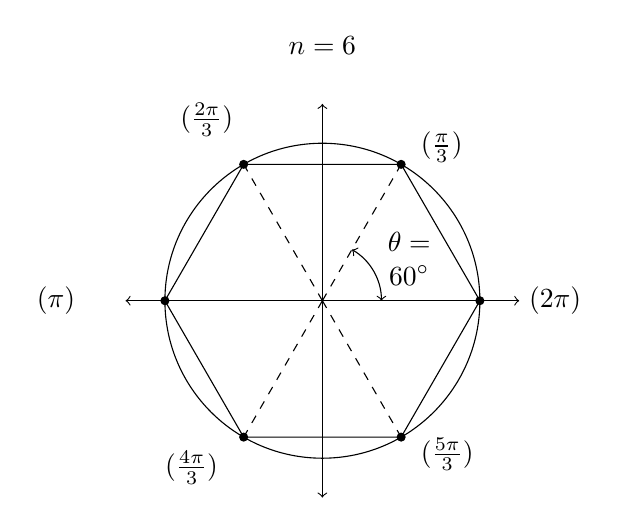
\begin{tikzpicture}[scale=1]

\draw [<->]  (0,-2.5) -- (0,2.5);
\draw  [<->] (-2.5,0) -- (2.5,0);

\draw (0,0) circle  (2);

\draw (0:2) \foreach \x in {60,120,...,359} {
                -- (\x:2)
            }-- cycle (90:2); 
\node[above] at (90:3) {$n=6$} ;

\draw[dashed] (0,0) -- (60:2);
\draw[dashed] (0,0) -- (120:2);
\draw[dashed] (0,0) -- (240:2);
\draw[dashed] (0,0) -- (300:2);

\draw[<->] (.75,0) arc (0:60:.75);
\node [right] at (45:.7) {\begin{tabular}{c} $\theta =$ \\ $60^{\circ}$ \end{tabular}};

\filldraw[fill=black, draw=black] (0:2) circle (0.05cm);
\node [right] at (0:2.5) {$\cis(2\pi)$};

\filldraw[fill=black, draw=black] (60:2) circle (0.05cm);
\node [right] at (60:2.25) {$\cis(\frac{\pi}{3})$};

\filldraw[fill=black, draw=black] (120:2) circle (0.05cm);
\node [right] at (130:3) {$\cis(\frac{2\pi}{3})$};

\filldraw[fill=black, draw=black] (180:2) circle (0.05cm);
\node [right] at (180:3.75) {$\cis(\pi)$};

\filldraw[fill=black, draw=black] (240:2) circle (0.05cm);
\node [right] at (225:3) {$\cis(\frac{4\pi}{3})$};

\filldraw[fill=black, draw=black] (300:2) circle (0.05cm);
\node [right] at (300:2.25) {$\cis(\frac{5\pi}{3})$};
\end{tikzpicture}
\end{center}
\end{figure}
Proposition \ref{proposition:complex:nth_roots_of_1} states the the $nth$ roots of unity are found by $\frac{2k\pi}{n}$, therefore the $6th$ roots of unity are $\frac{2k\pi}{6}$.  The above picture shows a hexagon with the $6th$ roots of unity. By drawing lines from the the $6th$ roots of unity to the center of the hexagon 6 triangles were created. To see if the hexagon is regular all triangles have to be congruent.\\
    
Each interior angle is $60^{\circ}$ and the sides to each triangle is a length of $1$ because the radius of the unit circle is $1$. Now we can say that all the triangles are congruent because of the side-angle-side(SAS) postulate. Therfore, all the sides forming the hexagon congruent and all the angles forming the hexagon are congruent. \\
    
Since all the sides and angles to the hexagon are congruent the hexagon is a regular hexagon.\\

\noindent\textbf{Exercise \ref{exercise:complex:hexagon_rotate}:} %kw added
\begin{enumerate}[(a)]
\item
%Draw a picture of the  6th roots of unity in the complex plane. Label them $A,B,C,D,E,F$ with $A=1, B= \cis\left(\frac{2\pi}{6}\right),$ and $C,D,E,F$ going counterclockwise around the circle. 
\begin{figure}[H]
\begin{center}
\tikzpreface{hexagon_rotate_a}
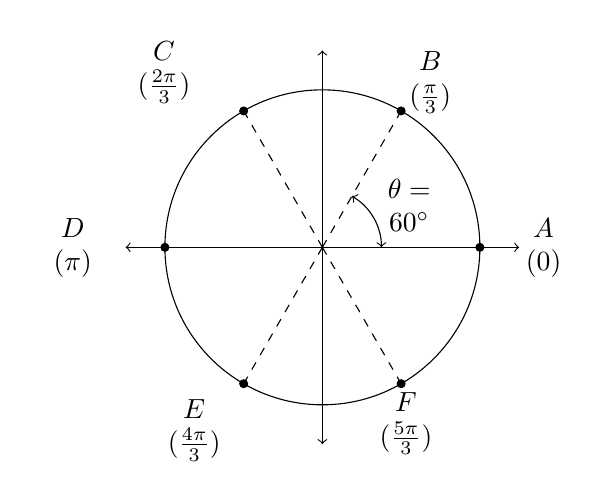
\begin{tikzpicture}[scale=1]

\draw [<->]  (0,-2.5) -- (0,2.5);
\draw  [<->] (-2.5,0) -- (2.5,0);

\draw (0,0) circle  (2);

\draw[dashed] (0,0) -- (60:2);
\draw[dashed] (0,0) -- (120:2);
\draw[dashed] (0,0) -- (240:2);
\draw[dashed] (0,0) -- (300:2);

\draw[<->] (.75,0) arc (0:60:.75);
\node [right] at (45:.7) {\begin{tabular}{c} $\theta =$ \\ $60^{\circ}$ \end{tabular}};

\filldraw[fill=black, draw=black] (0:2) circle (0.05cm);
\node [right] at (0:2.25) {\begin{tabular}{c} $A$ \\ $\cis(0)$ \end{tabular}};

\filldraw[fill=black, draw=black] (60:2) circle (0.05cm);
\node [right] at (70:2.25) {\begin{tabular}{c} $B$ \\ $\cis(\frac{\pi}{3})$ \end{tabular}};

\filldraw[fill=black, draw=black] (120:2) circle (0.05cm);
\node [right] at (140:3.5)  {\begin{tabular}{c} $C$ \\ $\cis(\frac{2\pi}{3})$ \end{tabular}};

\filldraw[fill=black, draw=black] (180:2) circle (0.05cm);
\node [right] at (180:3.75) {\begin{tabular}{c} $D$ \\ $\cis(\pi)$ \end{tabular}};

\filldraw[fill=black, draw=black] (240:2) circle (0.05cm);
\node [right] at (225:3.25) {\begin{tabular}{c} $E$ \\ $\cis(\frac{4\pi}{3})$ \end{tabular}};

\filldraw[fill=black, draw=black] (300:2) circle (0.05cm);
\node [right] at (280:2.25) {\begin{tabular}{c} $F$ \\ $\cis(\frac{5\pi}{3})$ \end{tabular}};
\end{tikzpicture}
\end{center}
\end{figure}

\item
%Fill in each of the following blanks with the letter corresponding to the product of the two complex numbers. For example,  $B \cdot B = \cis\left(\frac{2\pi}{6}\right) \cdot \cis\left(\frac{2\pi}{6}\right) = \cis\left(\frac{2\pi}{3}\right) = C$.
	\begin{enumerate}[(1)]
	\item
	%$B \cdot A = \underline{~<1>~}$
	$\cis(\frac{2\pi}{6})\cdot 1 = \cis(\frac{\pi}{3}) = B$\\

	\item
	%$B \cdot B = \underline{~<2>~}$ 
	$\cis\left(\frac{2\pi}{6}\right)\cdot \cis\left(\frac{2\pi}{6}\right) = \cis			\left(\frac{2\pi}{3}\right) = C$\\

	\item
	%$B \cdot C = \underline{~<3>~}$
	$\cis(\frac{2\pi}{6})\cdot \cis(\frac{4\pi}{6}) = \cis(\pi) = -1 = D$\\

	\item
	%$B \cdot D = \underline{~<4>~}$
	$\cis(\frac{2\pi}{6})\cdot(-1) = -\cis(\frac{2\pi}{6}) = \cis(\frac{4\pi}				{3}) = E$\\

	\item
	%$B \cdot E = \underline{~<5>~}$ 
	$\cis(\frac{2\pi}{6})\cdot \cis(\frac{8\pi}{6}) = \cis(\frac{5\pi}{3}) = F$		\\

	\item
	%$B \cdot F = \underline{~<6>~}$
	$\cis(\frac{2\pi}{6})\cdot \cis(\frac{10\pi}{6}) = \cis(2\pi) = 1 = A$
	\end{enumerate}

\item
%Using your answers from part (b), on your picture draw an arrow from $A$ to $B \cdot A$; similarly draw arrows from $B$ to $B \cdot B$, $C$ to $B \cdot C$, and so on. What do you observe about the arrows?
\begin{figure}[H]
\begin{center}
\tikzpreface{hexagon_rotate_c}
\begin{tikzpicture}[scale=1]

\draw [<->]  (0,-2.5) -- (0,2.5);
\draw  [<->] (-2.5,0) -- (2.5,0);

\draw (0,0) circle  (2);

\draw[-{Latex}] (0:2) -- (60:2);
\draw[-{Latex}] (60:2) -- (120:2);
\draw[-{Latex}] (120:2) -- (180:2);
\draw[-{Latex}] (180:2) -- (240:2);
\draw[-{Latex}] (240:2) -- (300:2);
\draw[-{Latex}] (300:2) -- (0:2);

\filldraw[fill=black, draw=black] (0:2) circle (0.05cm);
\node [right] at (0:2.25) {\begin{tabular}{c} $A$ \\ $\cis(0)$ \end{tabular}};

\filldraw[fill=black, draw=black] (60:2) circle (0.05cm);
\node [right] at (70:2.25) {\begin{tabular}{c} $B$ \\ $\cis(\frac{\pi}{3})$ \end{tabular}};

\filldraw[fill=black, draw=black] (120:2) circle (0.05cm);
\node [right] at (140:3.5)  {\begin{tabular}{c} $C$ \\ $\cis(\frac{2\pi}{3})$ \end{tabular}};


\filldraw[fill=black, draw=black] (180:2) circle (0.05cm);
\node [right] at (180:3.75) {\begin{tabular}{c} $D$ \\ $\cis(\pi)$ \end{tabular}};

\filldraw[fill=black, draw=black] (240:2) circle (0.05cm);
\node [right] at (225:3.25) {\begin{tabular}{c} $E$ \\ $\cis(\frac{4\pi}{3})$ \end{tabular}};

\filldraw[fill=black, draw=black] (300:2) circle (0.05cm);
\node [right] at (280:2.25) {\begin{tabular}{c} $F$ \\ $\cis(\frac{5\pi}{3})$ \end{tabular}};
\end{tikzpicture}
\end{center}
\end{figure}
The hexagon is rotating $\frac{\pi}{3}=B$ units.\\
 
\item
%It appears that multiplying all of the corners of the hexagon $ABCDEF$ by $B$ produces a \emph{rotation} of the hexagon. What is the angle of rotation?
The angle of rotation of the hexagon is $\frac{\pi}{3}$ or $60^{\circ}$.\\

\item
%Fill in the blanks:
	\begin{enumerate}[(1)]
	\item
	%$E \cdot A = \underline{~<1>~}$
	$\cis(\frac{4\pi}{3})\cdot 1 = \cis(\frac{4\pi}{3}) = E$

	\item
	%$E \cdot B = \underline{~<2>~}$
	$\cis(\frac{4\pi}{3})\cdot \cis(\frac{\pi}{3}) = \cis(\frac{5\pi}{3}) = F$

	\item
	%$E \cdot C = \underline{~<3>~}$
	$\cis(\frac{4\pi}{3})\cdot \cis(\frac{2\pi}{3}) = \cis(2\pi) = 1 = A$

	\item
	%$E \cdot D = \underline{~<4>~}$
	$\cis(\frac{4\pi}{3})\cdot \cis(\pi) = \cis(\frac{7\pi}{3}) = B$ 

	\item
	%$E \cdot E = \underline{~<5>~}$
	$\cis(\frac{4\pi}{3})\cdot \cis(\frac{4\pi}{3}) = \cis(\frac{8\pi}{3}) = C$

	\item
	%$E \cdot F = \underline{~<6>~}$.
	$\cis(\frac{4\pi}{3})\cdot \cis(\frac{5\pi}{3}) = \cis(3\pi) = D$
	\end{enumerate}

\item 
%Just as in part (c), use your answers from part (d) to draw arrows from $A$ to $E \cdot A$, $B$ to $E \cdot B$, etc. What do you observe about the arrows? 
\begin{figure}[H]
\begin{center}
\tikzpreface{hexagon_rotate_f}
\begin{tikzpicture}[scale=1]

\draw [<->]  (0,-2.5) -- (0,2.5);
\draw  [<->] (-2.5,0) -- (2.5,0);

\draw (0,0) circle  (2);

\draw[-{Latex}] (0:2) -- (240:2);  
\draw[-{Latex}] (60:2) -- (300:2);   
\draw[-{Latex}] (120:2) -- (0:2);   
\draw[-{Latex}] (180:2) -- (60:2);   
\draw[-{Latex}] (240:2) -- (120:2);   
\draw[-{Latex}] (300:2) -- (180:2);     

\filldraw[fill=black, draw=black] (0:2) circle (0.05cm);
\node [right] at (0:2.25) {\begin{tabular}{c} $A$ \\ $\cis(0)$ \end{tabular}};

\filldraw[fill=black, draw=black] (60:2) circle (0.05cm);
\node [right] at (70:2.25) {\begin{tabular}{c} $B$ \\ $\cis(\frac{\pi}{3})$ \end{tabular}};

\filldraw[fill=black, draw=black] (120:2) circle (0.05cm);
\node [right] at (140:3.5)  {\begin{tabular}{c} $C$ \\ $\cis(\frac{2\pi}{3})$ \end{tabular}};


\filldraw[fill=black, draw=black] (180:2) circle (0.05cm);
\node [right] at (180:3.75) {\begin{tabular}{c} $D$ \\ $\cis(\pi)$ \end{tabular}};

\filldraw[fill=black, draw=black] (240:2) circle (0.05cm);
\node [right] at (225:3.25) {\begin{tabular}{c} $E$ \\ $\cis(\frac{4\pi}{3})$ \end{tabular}};

\filldraw[fill=black, draw=black] (300:2) circle (0.05cm);
\node [right] at (280:2.25) {\begin{tabular}{c} $F$ \\ $\cis(\frac{5\pi}{3})$ \end{tabular}};
\end{tikzpicture}
\end{center}
\end{figure}
The arrows rotate the hexagon by $\frac{4\pi}{3}=E$ units.

\item
	\begin{enumerate}[(1)]
	\begin{multicols}{3}
	%Fill in the blanks:  If you choose one particular 6th root of unity and 			multiply it with all the other 6th roots, the new values correspond to 				different 
	\item
	%$\underline{~<1>~}$ of the original hexagon. 
	$6th$ roots of unity

	\item
	%The angle of $\underline{~<2>~}$ 
	roots of unity

	\item
	%is equal to the complex argument of the $\underline{~<3>~}$.
	chosen $6th$ root of unity
	\end{multicols}
	\end{enumerate}
\end{enumerate}

\noindent\textbf{Exercise \ref{exercise:complex:55}:} %kw added
\begin{enumerate}[(a)]
\item
%Just as in part (b) of Exercise~\ref{exercise:complex:hexagon_rotate} fill in the blanks with the correct letter $A,B,C,D,E$ or $F$ (recall that $\overline{A}$ denotes the complex conjugate of $A$).
	\begin{enumerate}[(1)]
	\begin{multicols}{3}
	\item
	%$ \overline{A} = \underline{~<1>~} $
	A
	
	\item
	%$  \overline{B} = \underline{~<2>~}$
	F
	
	\item
	%$  \overline{C} = \underline{~<3>~}$
	E
	
	\item
	% $ \overline{D} = \underline{~<4>~}$
	D
	
	\item
	%$ \overline{E} = \underline{~<5>~}$
	C
	
	\item
	% $ \overline{F} = \underline{~<6>~}).  $
	B
	\end{multicols}
	\end{enumerate}
	
\item 
%Just as in part (c) of Exercise~\ref{exercise:complex:hexagon_rotate}, draw arrows from $A$ to $\overline{A}$, $B$ to $\overline{B}$, etc. What do you observe about the arrows?
\begin{figure}[H]
\begin{center}
\tikzpreface{55b}
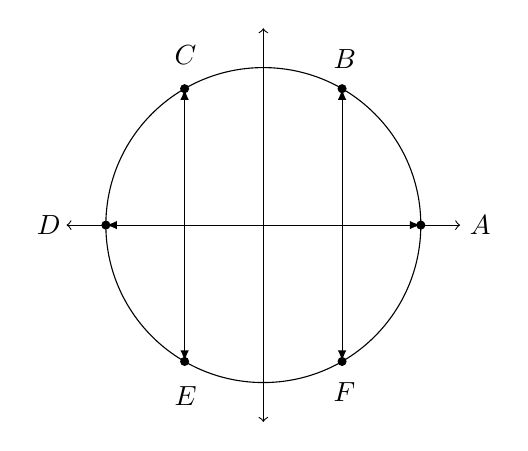
\begin{tikzpicture}[scale=1]

\draw [<->]  (0,-2.5) -- (0,2.5);
\draw  [<->] (-2.5,0) -- (2.5,0);

\draw (0,0) circle  (2);

\draw[-{latex}] (0:2) -- (180:2);  
\draw[-{latex}] (60:2) -- (300:2);   
\draw[-{latex}] (120:2) -- (240:2);   
\draw[-{latex}] (180:2) -- (0:2);   
\draw[-{latex}] (240:2) -- (120:2);   
\draw[-{latex}] (300:2) -- (60:2);     

\filldraw[fill=black, draw=black] (0:2) circle (0.05cm);
\node [right] at (0:2.5) {$A$};

\filldraw[fill=black, draw=black] (60:2) circle (0.05cm);
\node [right] at (70:2.25) {$B$};

\filldraw[fill=black, draw=black] (120:2) circle (0.05cm);
\node [right] at (120:2.5)  {$C$};

\filldraw[fill=black, draw=black] (180:2) circle (0.05cm);
\node [right] at (180:3) {$D$};

\filldraw[fill=black, draw=black] (240:2) circle (0.05cm);
\node [right] at (240:2.5) {$E$};

\filldraw[fill=black, draw=black] (300:2) circle (0.05cm);
\node [right] at (290:2.25) {$F$};
\end{tikzpicture}
\end{center}
\end{figure}
The area from one point, points to the corner that is straight across from it over the real axis.

\item 
%We refer to the geometrical motion produced by complex conjugation as ``flipping". What is the axis of the ``flip'' that is produced by taking the complex conjugates of the sixth roots of unity?
The real axis.
\end{enumerate}

\noindent\textbf{Exercise \ref{exercise:complex:non_comm}:} %kw added
\begin{enumerate}[(a)]
\item 
%What geometrical motion corresponds to the following algebraic operation:
%Multiply all 6th roots by $D$, then take the complex conjugates.
Flip around the imaginary axis.

\item 
%What geometrical motion corresponds to the following algebraic operation:
%``Take the complex conjugates of all 6th roots, then multiply by  $D$.''

\item 
%What geometrical motion corresponds to the following algebraic operation:
%``Multiply all 6th roots by $C$, then take the complex conjugates.''
Flip around the $\theta = \frac{2\pi}{3}$ axis.

\item 
%What geometrical motion corresponds to the following algebraic operation:
%``Take the complex conjugates of all 6th roots, then multiply by  $C$.''

\end{enumerate}

\noindent\textbf{Exercise \ref{exercise:complex:56}:}

\noindent\textbf{Exercise \ref{exercise:complex:57}:}

\noindent\textbf{Exercise \ref{exercise:complex:58}:}

\noindent\textbf{Exercise \ref{exercise:complex:58a}:}

\noindent\textbf{Exercise \ref{exercise:complex:59}:}

\noindent\textbf{Exercise \ref{exercise:complex:60}:} %kw added
%(In this exercise, you may leave your answers in polar form)
\begin{enumerate}[(a)]
\item
%Find all fifth roots of $-i$.
	$\cis(\frac{(3+4k)\pi }{10})$
\item
%Find all fourth roots of $-1 + \sqrt{3}i$.
$2^{1/4} \cis (\frac{\pi(1+3k)}{6})$
\item
%Find all fourth roots of $ \sqrt{1/2 + \sqrt{2}/4} + i\sqrt{1/2 - \sqrt{2}/4}$. 
%\hyperref[sec:complex:hints]{(*Hint*)}
	$\cis(\frac{\pi(1+8k)}{16})$
\item
%Find all sixth roots of $-16i$.
\item
$2^{1/3} \cis ( \frac{\pi}{4} + \frac{k\pi}{3} )$

\end{enumerate}

\noindent\textbf{Exercise \ref{exercise:complex:60a}:} 

\noindent\textbf{Exercise \ref{exercise:complex:cubic_conj}:} %kw added
%Consider the cubic equation $z^3 + pz^2 + qz = r$, where $p, q$ and  $r$ are all real numbers.
\begin{enumerate}[(a)]
\item
%Using an appropriate identity from Exercise \ref{exercise:complex:cxprops}, show that $\overline{z^3} = \overline{z}^3$.
	\begin{align*}
	(\overline{z})^{3} &		&\text{(Premise)}\\
	\overline{z}\overline{w} &= \overline{zw}	&\text{(Exercise 									\ref{exercise:complex:cxprops}b)}\\
	z &= a + bi 		&\text{(Given)}\\
	\overline{z} &= a - bi		&\text{(Def. of complex conjugate)}\\
	\overline{z} \cdot \overline{z} &= (a - bi)(a - bi)		&\text{(multiply by}\ 		\overline{z})\\
	\overline{z}^{2} &= (a^{2} - b^{2}) + (-ab -2b)i		&\text{(complex 				multiplication)}\\
	 &= (a^{2} - b^{2}) + (-2ab)i		&\text{(additive inverse)}\\
	 \overline{z} \cdot \overline{z}^{2} &= (a - bi)[(a^{2} - b^{2}) + 					(-2ab)i]		&\text{(multiply by}\ \overline{z})\\
	 \overline{z}^{3} &= [(a(a^{2} - b^{2}) - 2ab^{2}) + (-2a^{2}b -b(a^{2} - b^{2}))i]		&\text{(complex multiplication)}\\
	 \overline{z} \cdot \overline{z^{2}} &= (\overline{z})^{3} &\text{(Exercise 									\ref{exercise:complex:cxprops}b)}\\
	 \overline{z} \cdot \overline{z} \cdot \overline{z} &= (\overline{z})^{3} &\text{(Substitution)}\\
	 \\
	 (\overline{z^{3}})& &\text{(Premise)}\\
	 (\overline{z \cdot z^{2}})&   &\text{(basic algebra)}\\
	 \overline{z} \cdot \overline{z^{2}}&   &\text{(Exercise 									\ref{exercise:complex:cxprops}b)}\\
	 \overline{z} \cdot \overline{z} \cdot \overline{z}&    &\text{(Exercise 									\ref{exercise:complex:cxprops}b)}\\
	 (\overline{z})^{3}&   &\text{(basic algebra)}\\
	 \\
	 \therefore (\overline{z})^{3} &= (\overline{z^{3}}) &\text{(Conclusion)}
	\end{align*}
	
\item
%Similarly, show  $\overline{pz^2} = p\overline{z}^2$ and $\overline{qz} = q\overline{z}$, and $\overline{r} = r$.
	\begin{align*}
	\overline{pz^{2}}&= p(\overline{z})^{2}		&\text{(Premise, where}\ p \in {\mathbb{R}})\\
	a\overline{z}&= \overline{az}	&\text{(Given, where}\ a \in {\mathbb{R}})\\
	p(\overline{z})^{2}&= p(\overline{z^{2}}) &\text{(Exercise \ref{exercise:complex:cubic_conj}a)}\\
	&= \overline{pz^{2}} &\text{(Exercise \ref{exercise:complex:cxprops}e)}\\
	\therefore \overline{pz^{2}} &= p(\overline{z})^{2} &\text{(Conclusion)}\\
	\\
	\overline{az}&= a\overline{z}		&\text{(Premise, where}\ a \in {\mathbb{R}})\\
	a\overline{z}&= \overline{az}	&\text{(Given, where}\ a \in {\mathbb{R}})\\
	a\overline{z}& &\text{(Right side of premise)}\\
	\overline{az}& &\text{(Exercise \ref{exercise:complex:cxprops}e)}\\
	\therefore \overline{az} &= a\overline{z} &\text{(Conclusion)}\\
\\
	\overline{r}&= r	&\text{(Premise, where}\ r \in {\mathbb{R}})\\
	r&= r + 0&\text{(Additive Identity)}\\
	r&= r + 0i&\text{(Multiplication by by zero)}\\
	\overline{r}&= r - 0i &\text{(Def. of complex conjugate)}\\
	r&= r &\text{(Additive Identity)}\\
	\overline{r}&= r &\text{(Additive Identity)}\\
	\therefore \overline{r} &= r &\text{(Conclusion)}\\
	\end{align*}
	
\item 
%Use (a) and (b) to show that $\overline{z^3 + pz^2 + qz - r} = \overline{z}^3 + p\overline{z}^2 + q\overline{z} - r$.
	\begin{align*}
	\overline{z^{3} + pz^{2} + qz - r} &= \overline{z}^{3} + p\overline{z}^{2} + q\overline{z} - r    &\text{(Premise)}\\
	\overline{z^{3} + pz^{2} + qz - r} & &\text{(LHS of premise)}\\
	\overline{(z^{3} + pz^{2}) + (qz - r)} & &\text{(Additive \& associative of}\ {\mathbb{C}})\\
	\overline{(z^{3} + pz^{2})} + \overline{(qz - r)} & &\text{(Proposition \ref{proposition:complex:conj_add})}\\
	\overline{(z^{3} + pz^{2})} + \overline{(qz + (-r))} & &\text{(Additive Inverse)}\\
	(\overline{z^{3}} + \overline{pz^{2}}) + (\overline{qz} + \overline{(-r)})& &\text{(Proposition \ref{proposition:complex:conj_add})}\\
	\overline{z^{3}} + \overline{pz^{2}} + \overline{qz} + \overline{(-r)}& &\text{(Additive \& associative of}\ {\mathbb{C}})\\
	\overline{z}^{3}+ \overline{pz^{2}} + \overline{qz} + \overline{(-r)}& &\text{(Exercise \ref{exercise:complex:cubic_conj}a)}\\
	\overline{z}^{3}+ p\overline{z}^{2} + q\overline{z} + \overline{(-1)r}& &\text{(Exercise \ref{exercise:complex:cubic_conj}b)}\\
	\overline{z}^{3}+ p\overline{z}^{2} + q\overline{z} - r& &\text{(Exercise \ref{exercise:complex:cubic_conj}b)}\\
	\therefore \overline{z^{3} + pz^{2} + qz - r} &= \overline{z}^{3} + p\overline{z}^{2} + q\overline{z} - r &\text{(Conclusion)}\\
	\end{align*}	
	
\item
%Using (c), show that $z^3 + pz^2 + qz - r = 0$ implies that $\overline{z}^3 + p\overline{z}^2 + q\overline{z} - r = 0$.
\item
%Using (d), show that if $z$ is a solution to $z^3 + pz^2 + qz = r$ then $\overline{z}$ is also a solution.
\end{enumerate}

\noindent\textbf{Exercise \ref{exercise:complex:conjugate_root2a}:}\\ %kw added
%Suppose the cubic equation $z^3 + pz^2 + qz = r$ has an odd number of solutions. Show that at least one of the solutions must be real.
The cubic equation has a degree of $3$, which means there must be three solutions. Suppose $z$ is a solution to the equation $z^{3} + pz^{2} + qz - r = 0$.  
\begin{align*}
z^{3} + pz^{2} + qz &= r &\text{(Given)}\\
z^{3} + pz^{2} + qz - r&= 0 &\text{(Additive inverse)}\\
\end{align*}
From Exercise \ref{exercise:complex:cubic_conj}e, it was proven that $z^3 + pz^2 + qz - r = 0$, which implies that $\overline{z}^{3}+ p\overline{z}^{2} + q\overline{z} - r = 0$. This suggests that $z$ and $\overline{z}$ are two solutions to the cubic equation above. This leaves us with $z^3 + pz^2 + qz - r = 0$ having one more solution. Two options are one real solution or one complex solution. If there were another complex solution, $z_{0}$, then $\overline{z_{0}}$ also exists. This causes the cubic equation to have four solutions instead of three. Hence, there must be at least one real solution.
  
\noindent\textbf{Exercise \ref{exercise:complex:62}:} %kw added
\begin{enumerate}[(a)]
\item
%Given that $3 - 7i$ and $-2+i$ are solutions to an equation of the form $z^4 + a_{3}z^{3} + a_{2} z^{n-2}+ a_1 z + a_0 = 0$ where $a_0, a_1, a_2, a_3$ are real. Find two other solutions to the same equation.
$\overline{z} = 3 + 7i$ and $\overline{z} = -2 - i$

\item
%*Find $a_0, a_1, a_2, a_3$. 
%\hyperref[sec:complex:hints]{(*Hint*)}
	\begin{itemize}
	\item
	$a_{0} = 290$
	
	\item
	$a_{1} = 202$
	
	\item
	$a_{2} = 39$
	
	\item
	$a_{3} = -2$
	\end{itemize}
\end{enumerate}

\noindent\textbf{Exercise \ref{exercise:complex:conjugate_root2}:}

\noindent\textbf{Exercise \ref{exercise:complex:70}:}

\noindent\textbf{Exercise \ref{exercise:complex:72}:}

\noindent\textbf{Exercise \ref{exercise:complex:72a}:}

\noindent\textbf{Exercise \ref{exercise:complex:72b}:}

%section 2.5
%\noindent\textbf{Exercise \ref{exercise:complex:41}:}\\
%
%\noindent\textbf{Exercise \ref{exercise:complex:wave1}:}\\
%
%\noindent\textbf{Exercise \ref{exercise:complex:waves}:}\\
%
%\noindent\textbf{Exercise \ref{exercise:complex:42}:}\\
%
%\noindent\textbf{Exercise \ref{exercise:complex:43}:}\\
%
%\noindent\textbf{Exercise \ref{exercise:complex:44}:}\\
%
%\noindent\textbf{Exercise \ref{exercise:complex:45}:}\\
%
%\noindent\textbf{Exercise \ref{exercise:complex:46}:}\\
%
%\noindent\textbf{Exercise \ref{exercise:complex:47}:}\\
%
%\noindent\textbf{Exercise \ref{exercise:complex:mandelbrot}:}\\
%
%\noindent\textbf{Exercise \ref{exercise:complex:excel}:}